\section{Exercício 165}
% \begin{figure}[h]
% \begin{center}
% 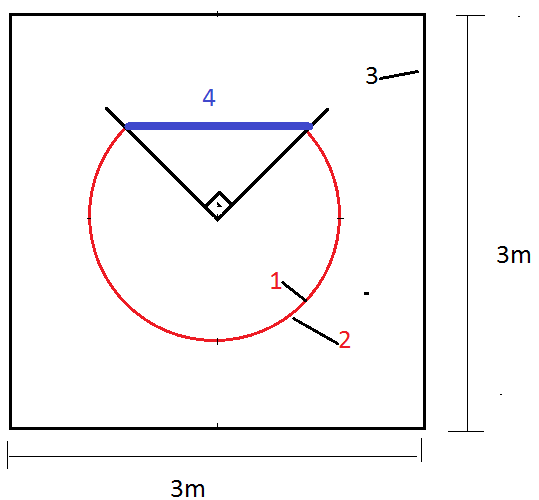
\includegraphics[scale=0.7]{./fig/1.png}
% \caption{\label{fig:1}1} 
% \end{center}
% \end{figure}

\myfig[scale=0.7]{figPME2321-20111121-01e}{1}

\pagebreak

% Table generated by Excel2LaTeX from sheet 'Plan1'
\begin{table}[htbp]
  \centering
  \caption{ Propriedades Termodinâmicas do Ciclo da Figura \ref{fig:1}}
    \begin{tabular}{rrrrrrr}
    \toprule
    Estagio & P(MPa) & T(K)  & v($m^{3}$/kg) & h(kJ/kg) & s(kJ/kg*K) & x \\
    \midrule
    1     & 0,007891 & 203   & 2.059 & 355   & 1,741 & 1 \\
    2     & 0,132700 & 253   & 0,1474 & 386,6 & 1,741 & 1 \\
    3     & 0,132700 & 253   & 0,1474 & 386,6 & 1,741 & 1 \\
    4     & 0,132700 & 253   & 0,1474 & 386,6 & 1,741 & 1 \\
    5     & 1,017000 & 313   & 0,01997 & 419,4 & 1,711 & 1 \\
    6     & 1,017000 & 313   & 0,000872 & 256,4 & 1,190 & 0 \\
    7     & 0,132700 & 253   & 0,05774 & 256,4 & 1,227 & 0,3887 \\
    8     & 0,132700 & 253   & 0,0007362 & 173,6 & 0,900 & 0 \\
    9     & 0,007981 & 203   & 0,5274 & 173,6 & 0,933 & 0,2559 \\
    \bottomrule
    \end{tabular}%
  \label{tab:1}%
\end{table}%

% \begin{figure}[h]
% \begin{center}
% 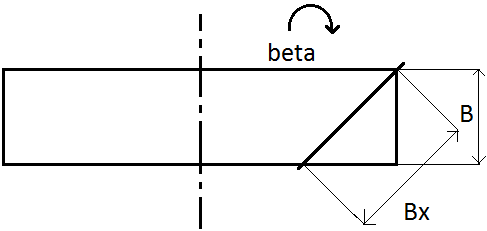
\includegraphics[scale=0.4]{./fig/4.png}
% \caption{\label{fig:4}Grafico T x s do ciclo da figura \ref{fig:1}} 
% \end{center}
% \end{figure}

\myfig[scale=0.4]{figPME2321-20111121-04e}{Grafico $T \times s$ do ciclo da figura \ref{figPME2321-20111121-01e}}


\subsection{a}

\begin{equation}
\beta = \frac{ -\dot{q}_{L}  }{ -\dot{w_{1}} - \dot{w_{2}} }
\label{eq:1}
\end{equation}

Considerando os compressores isentrópicos, temos que:
Para o compressor 1,
\[w_{1} = h_{2} - h_{1}\]
Consultando a tabela \ref{tab:1}, temos:

\[w_{1} = 386.6 - 355 = 31.6 kJ/kg\]
Para o compressor 2,
\[w_{2} = h_{5} - h_{4}\]
Consultando a tabela \ref{tab:1}, temos:

\[w_{2} = 419.4 - 386.6 = 32.8 kJ/kg\]

Para o evaporador, temos:
\[q_{L} = h_{1} - h_{9}\]
\[q_{L} = 355 - 173.6 = 181.4 kJ/kg\]

Logo, substituindo os valores na equação \ref{eq:1}, teremos:

\[\beta = \frac{ -\dot{q}_{L}  }{ -\dot{w_{1}} - \dot{w_{2}} }\]
\[\beta = \frac{ -181.4  }{ -31.6 - 32.8 } \]
\[\beta = 2.82\]

\pagebreak

\subsection{b}

% \begin{figure}[h]
% \begin{center}
% 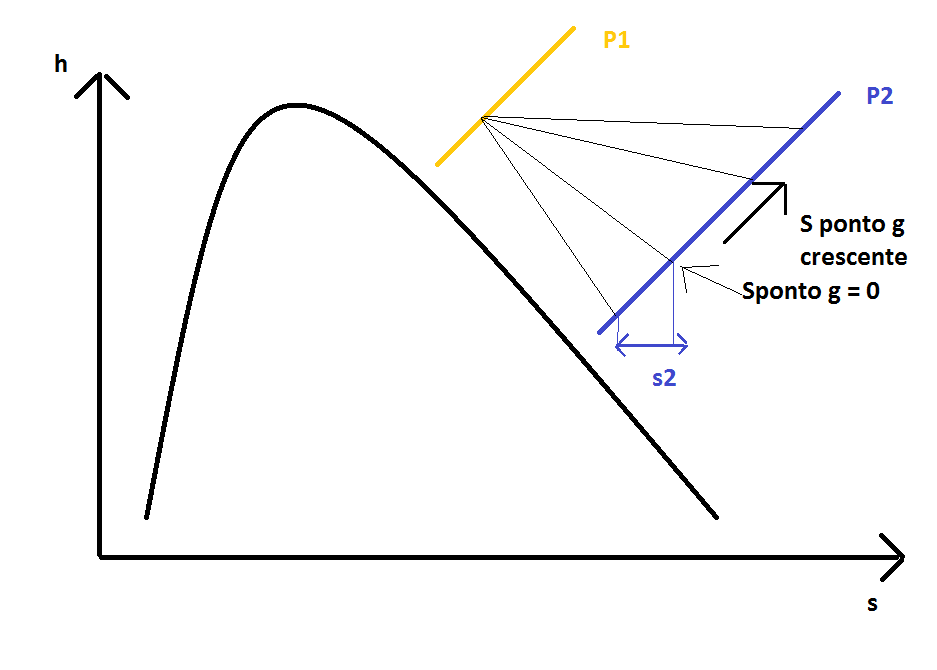
\includegraphics[scale=0.5]{./fig/2.png}
% \caption{\label{fig:2}Ciclo Ideal de Refrigeração} 
% \end{center}
% \end{figure}
\myfig[scale=0.5]{figPME2321-20111121-02e}{Ciclo Ideal de Refrigeração}


% \begin{figure}[h]
% \begin{center}
% 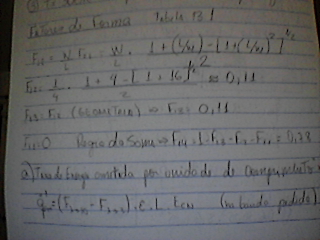
\includegraphics[scale=0.4]{./fig/3.png}
% \caption{\label{fig:3}Grafico T x s} 
% \end{center}
% \end{figure}

\myfig[scale=0.4]{figPME2321-20111121-03e}{Grafico $T \times s$}

% Table generated by Excel2LaTeX from sheet 'Plan2'
\begin{table}[htbp]
  \centering
  \caption{Propriedades termodinãmicas do ciclo simplificado do item b}
    \begin{tabular}{rrrrrrr}
    \toprule
    Estagio & P(MPa) & T(K)  & v($m^{3}$/kg) & h(kJ/kg) & s(kJ/kg*K) & x \\
    \midrule
    1     & 0,007891 & 203   & 2.059 & 355   & 1,741 & 1 \\
    2     & 1,017000 & 313   & 0,01997 & 419,4 & 1,711 & 1 \\
    3     & 1,017000 & 313   & 0,000872 & 256,4 & 1,190 & 0 \\
    4     & 0,007981 & 203   & 1,226 & 256,4 & 1,341 & 0,5955 \\
    \bottomrule
    \end{tabular}%
  \label{tab:2}%
\end{table}%

Considerando o compressor isentrópico, temos que:
Para o compressor ,
\[w_{1} = h_{2} - h_{1}\]
Consultando a tabela \ref{tab:2}, temos:

\[w_{1} = 419.4 - 355 = 64.4 kJ/kg\]

Para o evaporador, temos:
\[q_{L} = h_{1} - h_{4}\]
\[q_{L} = 355 - 256.4 = 98.6 kJ/kg\]

Logo, substituindo os valores na equação \ref{eq:1}, teremos:

\[\beta = \frac{ -\dot{q}_{L}  }{ -\dot{w_{1}} - \dot{w_{2}} }\]
\[\beta = \frac{ -98.6  }{ -64.4 } \]
\[\beta = 1.53\]

\paragraph*{Comentário}
O valor de $\beta$ do item $a)$ é maior do que o valor de $\beta$ no item $b)$ porque a "amplitude" ou diferença entre os valores de entalpia na entrada e na saída do evaporador (que constitui a parcela $q_{L}$ de $\beta$) é uma diferença maior em $a)$ do que em $b)$. Isso se deve ao fato de o ciclo separar a fase líquida da fase vapor em $7$ (flash chamber). Assim, uma maior fase de líquido vai para o evaporador, obtendo melhor rendimento.